%%=============================================================================
%% Vergelijkende studie
%%=============================================================================

\chapter{\IfLanguageName{dutch}{Vergelijkende studie}{Vergelijkende studie}}%
\label{ch:Vergelijkende studie}

In dit hoofdstuk zullen we de spraakmodellen die geselecteerd zijn in de short list vergelijken met elkaar. Deze worden geïmplementeerd op de nieuwste versie van het besturingssysteem Android. We evalueren deze modellen op basis van diverse criteria, waaronder:

\begin{itemize}
  \item Documentatie
  \item Implementatie
  \item Performantie
  \item Accuraatheid
  \item Taalondersteuning
  \item Kostprijs
\end{itemize}

Deze vergelijking zal ons in staat stellen de sterktes en zwaktes van elk model te identificeren en zo het meest geschikte spraakmodel voor het onderzoek te selecteren.

\section{Vosk}
Vosk is een open-source spraakherkenningstechnologie die een toolkit aanbiedt voor het ontwikkelen van spraakherkenning in applicaties. Het maakt gebruik van algoritmes van Kaldi, een toolkit voor spraakherkenning die ontwikkeld is in de programmeertaal C++, maar is geoptimaliseerd voor ontwikkelaars die spraakherkenning willen integreren in hun applicaties. Het model kan als geïntegreerde oplossing gebruikt worden in Android smartphones. Het ondersteund meer dan 20 talen en dialecten waaronder Engels, Frans en Nederlands. Het biedt ook een API aan waarmee ontwikkelaars de keuze krijgen om de spraakherkenning lokaal of in de cloud te verwerken. Deze compacte oplossing vereist slechts 50Mb aan opslagruimte en gebruikt ongeveer 300Mb aan geheugen tijdens uitvoering. Naast de spraakherkenning biedt Vosk ook de mogelijkheid om aan spreker identificatie te doen \autocite{HafizMuhammad2022}.

\subsection{Documentatie}
De officiële documentatie van Vosk is beschikbaar op de website van Alpha Cephei, het bedrijf achter Vosk. De documentatie is uitgebreid en bevat een duidelijke uitleg per onderdeel. Doordat Vosk ondersteuning biedt voor meerdere programmeertalen en besturingssystemen is de officiële documentatie meer een toolkit dan een handleiding. De community van Vosk is actief over verschillende platformen zoals GitHub, Discord, Reddit, Twitter,... . De documentatie is beschikbaar in het Engels en is toegankelijk voor iedereen.

\subsection{Implementatie}
Voor de implementatie van Vosk wordt er gebruik gemaakt van de demo applicatie die beschikbaar is gemaakt door de ontwikkelaars van Vosk. Deze demo applicatie is een Android applicatie die gebruik maakt van Kaldi- en Vosk-bibliotheken. De demo is te vinden op GitHub via de volgende link:
\url{https://github.com/alphacep/vosk-android-demo}.\newline

Er wordt gebruik gemaakt van Android Studio om de applicatie te implementeren. Het project gebruikt Java als programmeertaal voor de mobiele applicatie. Bij het opstarten van de applicatie wordt er gevraagd om de permissie voor de microfoon toe te staan. De applicatie is in staat om spraakherkenning uit te voeren aan de hand van een geluidsfragment in het .wav-formaat. De microfoon van de smartphone kan ook gebruikt worden om spraakherkenning uit te voeren. De applicatie ziet er als volgt uit:
\begin{figure}[H]
  \centering
  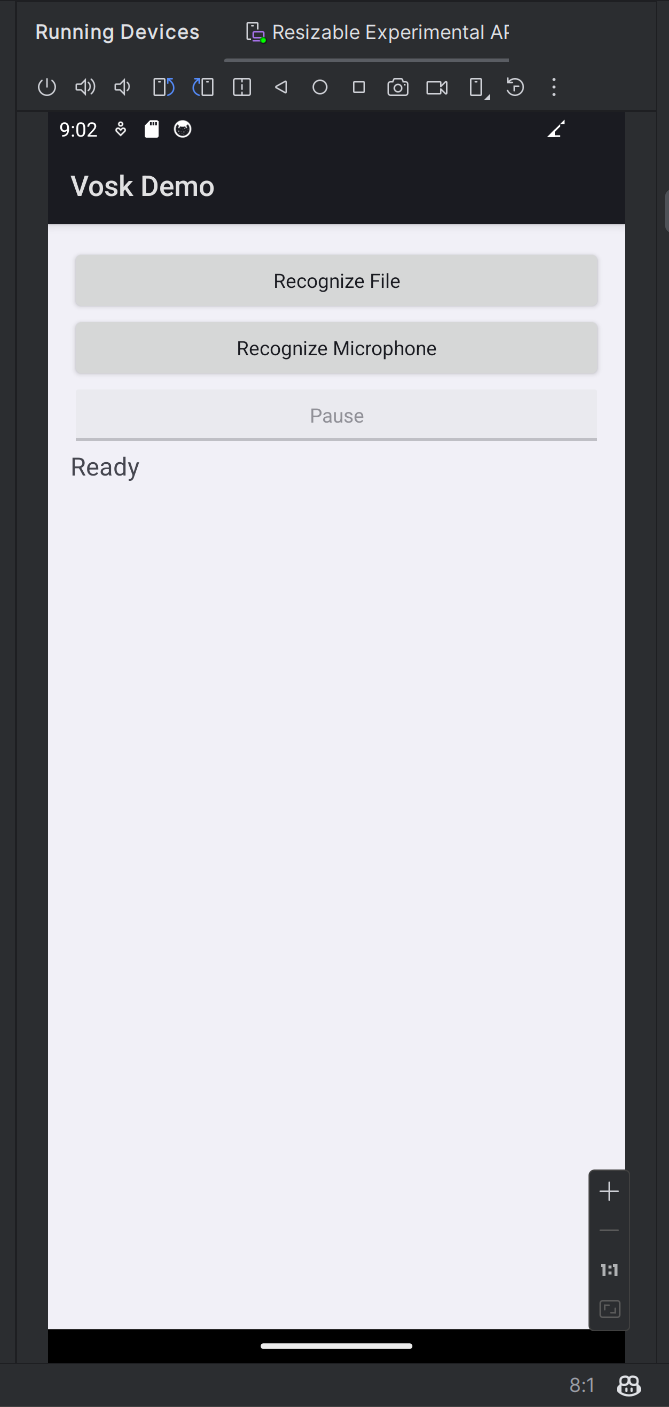
\includegraphics[scale=0.5]{Vosk_UI.png}
  \caption{UI van de Vosk demo applicatie}
\end{figure}

\subsection{Performantie}
De performantie van Vosk is afhankelijk van het gebruikte model. Vosk heeft per taal een groot en klein model. Het kleine model is ideaal voor bepaalde gelimiteerde toepassingen en heeft een grootte van ongeveer 50Mb. Het gebruikt ongeveer 300Mb aan geheugen tijdens de uitvoering, wat een ideaal model is voor mobiele toepassingen. Het grote model is ideaal voor toepassingen die een hogere accuraatheid vereisen. Dit model heeft een grootte van ongeveer 16Gb aan geheugen doordat het gebruik maakt van geavanceerde AI-algoritmes. Het nadeel van dit type model is dat de hardware krachtig genoeg moet zijn om de spraakherkenning uit te voeren. De ideale hardware voor dit model is een krachtige server, uitgerust met een Intel i7-processor of de nieuwste generatie AMD Ryzen-processoren. Het onderzoek richt zich op de talen Engels, Frans en Nederlands, waardoor er voor elke taal één specifiek spraakmodel is geselecteerd, in totaal dus drie spraakmodellen. Er is telkens gekozen voor het kleine model van Vosk, aangezien dit model ideaal is voor mobiele toepassingen. 
Volgende modellen worden gebruikt:

\begin{center}
  \begin{tabular}{ | l | l | l | p{5cm} |}
  \hline
  Modelnaam & Taalondersteuning & Grootte & Extra uitleg \\ \hline
  vosk-model-small-en-us-0.15 & US Engels & 40Mb & Klein model voor het Engels \\ \hline
  vosk-model-small-fr-0.22 & Frans & 41Mb & Klein model voor het Frans \\ \hline
  vosk-model-small-nl-0.22 & Nederlands & 39Mb & Klein model voor het Nederlands \\ \hline
  \end{tabular}
\end{center}

